\chapter{Evaluation}

\section{Event Detection Evaluation}
\subsection{Evaluation Data and Metric}
The evaluation for event detection uses data from IEEE AASP Challenge for event detection\footnote{http://c4dm.eecs.qmul.ac.uk/sceneseventschallenge}.  
In this challenge, a training dataset are given containing instantiations of individual events for 16 different classes. 
Moreover, there is also a developement dataset, which consist of 1 minute recordings of every-day audio events in a number of office environments. 
This developement dataset is annotated by human and can be used for model evaluation. \\ 

The evaluation begins by first segmenting clips using the a segmenter. 
We assume that only one event happens during a segment. 
Then use the trained GMM to calculate the posterior probability. 
The detected event is chosen when its corresponding GMM has the highest posterior probability.\\ 
 
Three types of assessment of the various systems will take place, i.e., a frame-based, event-based, and class-wise event-based evaluation \cite{giannoulis2013database}.  These three metrics differ mainly in the way they interpret a sequence result of detected events.  
Suppose $r$, $e$ and $c$ denotes number of ground truth, estimated and correct events, the Precision, Recall, and F-measure are defined as: 
\begin{equation}
	P = \frac{c}{e}, R = \frac{c}{r}, F = \frac{2PR}{P+R}.  
\end{equation}
For the frame-based metric, $r$, $e$, and $c$ are calculated in a 10ms window and are averaged over the entire duration. 
The event-based metric takes a different perspective of how a event unit is calculated. 
Unlike frame-based metric, which undiscriminately count event for every 10ms, this metric focuses on the true onset and offset time of ground truth events. 
Onset-only evaluation set restriction on onset time tolerance. 
Onset-offset evaluation further add a offset time restriction. 
The onset-only and onset-offset evaluation are averaged as event-based metric. 
Class-wise event-based calculate $r$, $e$, and $c$ for each class separately. And then it is averaged over classes. 
Finally, the F-measure for these three metric are averaged as the final metric of a system, and we will compare this metric with other systems. 

\subsection{Evaluation Process}
The evaluation takes on two parts: self tuning and system comparison. \\ 

Audio events are detected using the previous proposed GMM method, but there are still some parameters or configuration to be tuned for the best performance of our model.
Most importantly, the number of component number in GMM are ser by human, we run a evaluation for different component numbers from 4 to 45 to see how the number affects the F-measure. \\ 

In system comparison, we use other models from the aforementioned IEEE AASP Challenge\footnote{http://c4dm.eecs.qmul.ac.uk/sceneseventschallenge/resultsOL.html}. 
In the submitted papers, contestents also carried out the same evaluation on the developement dataset, so the comparison are done on the same dataset.  

\subsection{Evaluation Result}
\subsubsection{Component Number Evaluation}
Figure \ref{fig:component} is the result of average F-measure with regard to different component numbers in GMM. 
% component.eps
\begin{figure}[htb]
\centering
% GNUPLOT: LaTeX picture with Postscript
\begingroup
  \makeatletter
  \providecommand\color[2][]{%
    \GenericError{(gnuplot) \space\space\space\@spaces}{%
      Package color not loaded in conjunction with
      terminal option `colourtext'%
    }{See the gnuplot documentation for explanation.%
    }{Either use 'blacktext' in gnuplot or load the package
      color.sty in LaTeX.}%
    \renewcommand\color[2][]{}%
  }%
  \providecommand\includegraphics[2][]{%
    \GenericError{(gnuplot) \space\space\space\@spaces}{%
      Package graphicx or graphics not loaded%
    }{See the gnuplot documentation for explanation.%
    }{The gnuplot epslatex terminal needs graphicx.sty or graphics.sty.}%
    \renewcommand\includegraphics[2][]{}%
  }%
  \providecommand\rotatebox[2]{#2}%
  \@ifundefined{ifGPcolor}{%
    \newif\ifGPcolor
    \GPcolorfalse
  }{}%
  \@ifundefined{ifGPblacktext}{%
    \newif\ifGPblacktext
    \GPblacktexttrue
  }{}%
  % define a \g@addto@macro without @ in the name:
  \let\gplgaddtomacro\g@addto@macro
  % define empty templates for all commands taking text:
  \gdef\gplbacktext{}%
  \gdef\gplfronttext{}%
  \makeatother
  \ifGPblacktext
    % no textcolor at all
    \def\colorrgb#1{}%
    \def\colorgray#1{}%
  \else
    % gray or color?
    \ifGPcolor
      \def\colorrgb#1{\color[rgb]{#1}}%
      \def\colorgray#1{\color[gray]{#1}}%
      \expandafter\def\csname LTw\endcsname{\color{white}}%
      \expandafter\def\csname LTb\endcsname{\color{black}}%
      \expandafter\def\csname LTa\endcsname{\color{black}}%
      \expandafter\def\csname LT0\endcsname{\color[rgb]{1,0,0}}%
      \expandafter\def\csname LT1\endcsname{\color[rgb]{0,1,0}}%
      \expandafter\def\csname LT2\endcsname{\color[rgb]{0,0,1}}%
      \expandafter\def\csname LT3\endcsname{\color[rgb]{1,0,1}}%
      \expandafter\def\csname LT4\endcsname{\color[rgb]{0,1,1}}%
      \expandafter\def\csname LT5\endcsname{\color[rgb]{1,1,0}}%
      \expandafter\def\csname LT6\endcsname{\color[rgb]{0,0,0}}%
      \expandafter\def\csname LT7\endcsname{\color[rgb]{1,0.3,0}}%
      \expandafter\def\csname LT8\endcsname{\color[rgb]{0.5,0.5,0.5}}%
    \else
      % gray
      \def\colorrgb#1{\color{black}}%
      \def\colorgray#1{\color[gray]{#1}}%
      \expandafter\def\csname LTw\endcsname{\color{white}}%
      \expandafter\def\csname LTb\endcsname{\color{black}}%
      \expandafter\def\csname LTa\endcsname{\color{black}}%
      \expandafter\def\csname LT0\endcsname{\color{black}}%
      \expandafter\def\csname LT1\endcsname{\color{black}}%
      \expandafter\def\csname LT2\endcsname{\color{black}}%
      \expandafter\def\csname LT3\endcsname{\color{black}}%
      \expandafter\def\csname LT4\endcsname{\color{black}}%
      \expandafter\def\csname LT5\endcsname{\color{black}}%
      \expandafter\def\csname LT6\endcsname{\color{black}}%
      \expandafter\def\csname LT7\endcsname{\color{black}}%
      \expandafter\def\csname LT8\endcsname{\color{black}}%
    \fi
  \fi
  \setlength{\unitlength}{0.0500bp}%
  \begin{picture}(7200.00,5040.00)%
    \gplgaddtomacro\gplbacktext{%
      \csname LTb\endcsname%
      \put(946,704){\makebox(0,0)[r]{\strut{} 0}}%
      \csname LTb\endcsname%
      \put(946,1383){\makebox(0,0)[r]{\strut{} 0.1}}%
      \csname LTb\endcsname%
      \put(946,2061){\makebox(0,0)[r]{\strut{} 0.2}}%
      \csname LTb\endcsname%
      \put(946,2740){\makebox(0,0)[r]{\strut{} 0.3}}%
      \csname LTb\endcsname%
      \put(946,3418){\makebox(0,0)[r]{\strut{} 0.4}}%
      \csname LTb\endcsname%
      \put(946,4097){\makebox(0,0)[r]{\strut{} 0.5}}%
      \csname LTb\endcsname%
      \put(946,4775){\makebox(0,0)[r]{\strut{} 0.6}}%
      \csname LTb\endcsname%
      \put(1078,484){\makebox(0,0){\strut{} 0}}%
      \csname LTb\endcsname%
      \put(1714,484){\makebox(0,0){\strut{} 5}}%
      \csname LTb\endcsname%
      \put(2350,484){\makebox(0,0){\strut{} 10}}%
      \csname LTb\endcsname%
      \put(2986,484){\makebox(0,0){\strut{} 15}}%
      \csname LTb\endcsname%
      \put(3622,484){\makebox(0,0){\strut{} 20}}%
      \csname LTb\endcsname%
      \put(4259,484){\makebox(0,0){\strut{} 25}}%
      \csname LTb\endcsname%
      \put(4895,484){\makebox(0,0){\strut{} 30}}%
      \csname LTb\endcsname%
      \put(5531,484){\makebox(0,0){\strut{} 35}}%
      \csname LTb\endcsname%
      \put(6167,484){\makebox(0,0){\strut{} 40}}%
      \csname LTb\endcsname%
      \put(6803,484){\makebox(0,0){\strut{} 45}}%
      \put(176,2739){\rotatebox{-270}{\makebox(0,0){\strut{}Average F-measure}}}%
      \put(3940,154){\makebox(0,0){\strut{}Component Number}}%
    }%
    \gplgaddtomacro\gplfronttext{%
    }%
    \gplbacktext
    \put(0,0){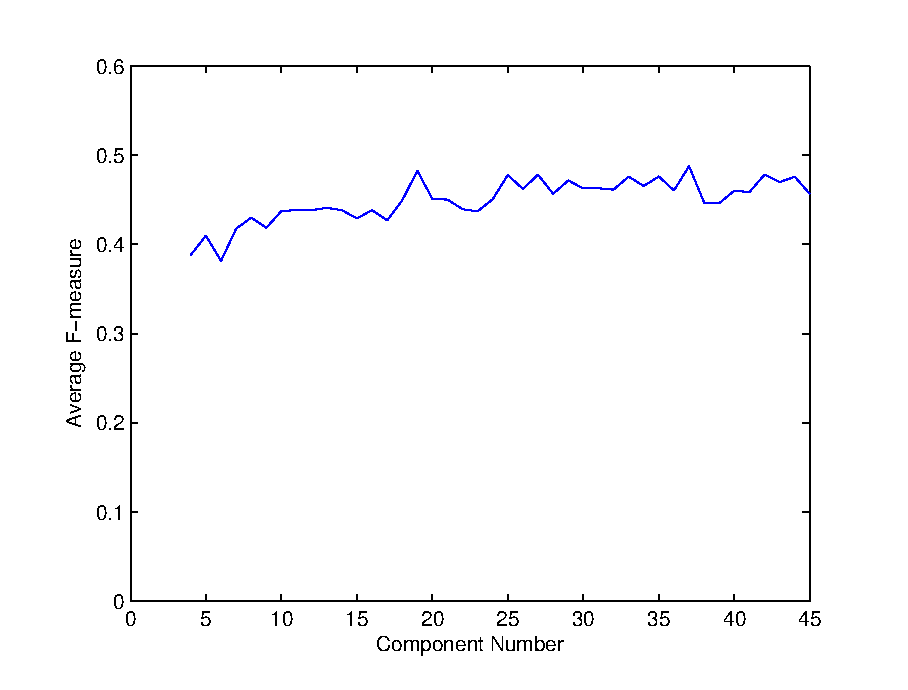
\includegraphics{component}}%
    \gplfronttext
  \end{picture}%
\endgroup

\caption{F-measure for different component number}
\label{fig:component}
\end{figure}

As we can see in Figure \ref{fig:component}, the F-measure gradually rise when component number are increasing. 
But after component number reaching 18 or so, the F-measure roughly stays the same. \\ 

% running time eps 
\begin{figure}[htb]
\centering
% GNUPLOT: LaTeX picture with Postscript
\begingroup
  \makeatletter
  \providecommand\color[2][]{%
    \GenericError{(gnuplot) \space\space\space\@spaces}{%
      Package color not loaded in conjunction with
      terminal option `colourtext'%
    }{See the gnuplot documentation for explanation.%
    }{Either use 'blacktext' in gnuplot or load the package
      color.sty in LaTeX.}%
    \renewcommand\color[2][]{}%
  }%
  \providecommand\includegraphics[2][]{%
    \GenericError{(gnuplot) \space\space\space\@spaces}{%
      Package graphicx or graphics not loaded%
    }{See the gnuplot documentation for explanation.%
    }{The gnuplot epslatex terminal needs graphicx.sty or graphics.sty.}%
    \renewcommand\includegraphics[2][]{}%
  }%
  \providecommand\rotatebox[2]{#2}%
  \@ifundefined{ifGPcolor}{%
    \newif\ifGPcolor
    \GPcolorfalse
  }{}%
  \@ifundefined{ifGPblacktext}{%
    \newif\ifGPblacktext
    \GPblacktexttrue
  }{}%
  % define a \g@addto@macro without @ in the name:
  \let\gplgaddtomacro\g@addto@macro
  % define empty templates for all commands taking text:
  \gdef\gplbacktext{}%
  \gdef\gplfronttext{}%
  \makeatother
  \ifGPblacktext
    % no textcolor at all
    \def\colorrgb#1{}%
    \def\colorgray#1{}%
  \else
    % gray or color?
    \ifGPcolor
      \def\colorrgb#1{\color[rgb]{#1}}%
      \def\colorgray#1{\color[gray]{#1}}%
      \expandafter\def\csname LTw\endcsname{\color{white}}%
      \expandafter\def\csname LTb\endcsname{\color{black}}%
      \expandafter\def\csname LTa\endcsname{\color{black}}%
      \expandafter\def\csname LT0\endcsname{\color[rgb]{1,0,0}}%
      \expandafter\def\csname LT1\endcsname{\color[rgb]{0,1,0}}%
      \expandafter\def\csname LT2\endcsname{\color[rgb]{0,0,1}}%
      \expandafter\def\csname LT3\endcsname{\color[rgb]{1,0,1}}%
      \expandafter\def\csname LT4\endcsname{\color[rgb]{0,1,1}}%
      \expandafter\def\csname LT5\endcsname{\color[rgb]{1,1,0}}%
      \expandafter\def\csname LT6\endcsname{\color[rgb]{0,0,0}}%
      \expandafter\def\csname LT7\endcsname{\color[rgb]{1,0.3,0}}%
      \expandafter\def\csname LT8\endcsname{\color[rgb]{0.5,0.5,0.5}}%
    \else
      % gray
      \def\colorrgb#1{\color{black}}%
      \def\colorgray#1{\color[gray]{#1}}%
      \expandafter\def\csname LTw\endcsname{\color{white}}%
      \expandafter\def\csname LTb\endcsname{\color{black}}%
      \expandafter\def\csname LTa\endcsname{\color{black}}%
      \expandafter\def\csname LT0\endcsname{\color{black}}%
      \expandafter\def\csname LT1\endcsname{\color{black}}%
      \expandafter\def\csname LT2\endcsname{\color{black}}%
      \expandafter\def\csname LT3\endcsname{\color{black}}%
      \expandafter\def\csname LT4\endcsname{\color{black}}%
      \expandafter\def\csname LT5\endcsname{\color{black}}%
      \expandafter\def\csname LT6\endcsname{\color{black}}%
      \expandafter\def\csname LT7\endcsname{\color{black}}%
      \expandafter\def\csname LT8\endcsname{\color{black}}%
    \fi
  \fi
  \setlength{\unitlength}{0.0500bp}%
  \begin{picture}(7200.00,5040.00)%
    \gplgaddtomacro\gplbacktext{%
      \csname LTb\endcsname%
      \put(1078,704){\makebox(0,0)[r]{\strut{} 400}}%
      \csname LTb\endcsname%
      \put(1078,1213){\makebox(0,0)[r]{\strut{} 600}}%
      \csname LTb\endcsname%
      \put(1078,1722){\makebox(0,0)[r]{\strut{} 800}}%
      \csname LTb\endcsname%
      \put(1078,2231){\makebox(0,0)[r]{\strut{} 1000}}%
      \csname LTb\endcsname%
      \put(1078,2740){\makebox(0,0)[r]{\strut{} 1200}}%
      \csname LTb\endcsname%
      \put(1078,3248){\makebox(0,0)[r]{\strut{} 1400}}%
      \csname LTb\endcsname%
      \put(1078,3757){\makebox(0,0)[r]{\strut{} 1600}}%
      \csname LTb\endcsname%
      \put(1078,4266){\makebox(0,0)[r]{\strut{} 1800}}%
      \csname LTb\endcsname%
      \put(1078,4775){\makebox(0,0)[r]{\strut{} 2000}}%
      \csname LTb\endcsname%
      \put(1210,484){\makebox(0,0){\strut{} 5}}%
      \csname LTb\endcsname%
      \put(1909,484){\makebox(0,0){\strut{} 10}}%
      \csname LTb\endcsname%
      \put(2608,484){\makebox(0,0){\strut{} 15}}%
      \csname LTb\endcsname%
      \put(3307,484){\makebox(0,0){\strut{} 20}}%
      \csname LTb\endcsname%
      \put(4006,484){\makebox(0,0){\strut{} 25}}%
      \csname LTb\endcsname%
      \put(4706,484){\makebox(0,0){\strut{} 30}}%
      \csname LTb\endcsname%
      \put(5405,484){\makebox(0,0){\strut{} 35}}%
      \csname LTb\endcsname%
      \put(6104,484){\makebox(0,0){\strut{} 40}}%
      \csname LTb\endcsname%
      \put(6803,484){\makebox(0,0){\strut{} 45}}%
      \put(176,2739){\rotatebox{-270}{\makebox(0,0){\strut{}Running Time (s)}}}%
      \put(4006,154){\makebox(0,0){\strut{}Component Number}}%
    }%
    \gplgaddtomacro\gplfronttext{%
    }%
    \gplbacktext
    \put(0,0){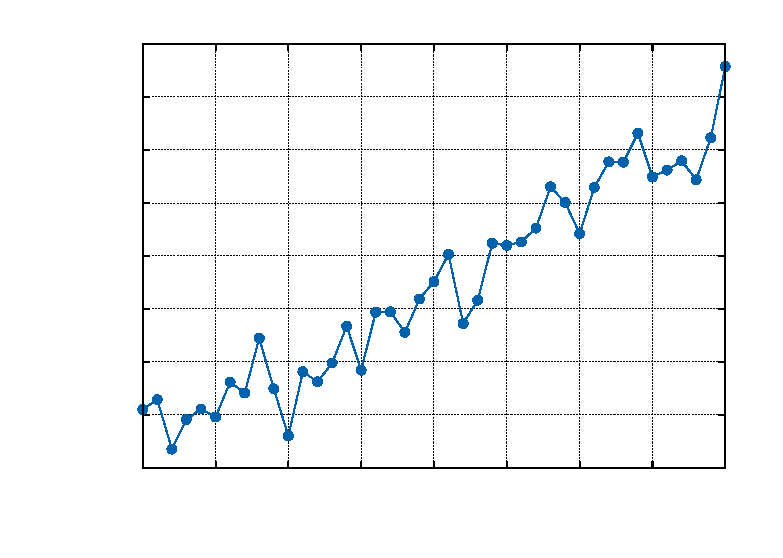
\includegraphics{componentTime}}%
    \gplfronttext
  \end{picture}%
\endgroup

\caption{Running time for different componet number}
\label{fig:componentTime}
\end{figure}
Moreover, Figure \ref{fig:componentTime} is the running time of our system with regard to the number of components. 
There is basically a linear relationship between the number of components and the total running time. 
Hence, we choose to use 18 as the component number for our system, since this component number has a good F-measure, and the speed for training models are also fast.\\ 

\subsubsection{Event Detection F-measure Evaluation}
\begin{table}[htb]
\centering
\caption{Event Detetion Evaluation}
\begin{tabular}{lllll}
\hline
         & EB    & CWEB  & FB    & Average \\
\hline
baseline & 15.4  & 13.5  & 20.6  & 16.50   \\
NR2      & 11.06 & 20.9  & 32.49 & 21.48   \\
NVM      & 47.53 & 41.28 & 54.41 & 47.74   \\
Our      & 53.44 & 40.07 & 52.41 & 48.64   \\
VVK      & 51.13 & 39.77 & 56.28 & 49.06   \\
GVV      & 46.8  & 36.7  & 65.2  & 49.57   \\
DHV      & 51.05 & 38.05 & 61.6  & 50.23   \\     
\hline
\end{tabular}
\end{table}
There are seven systems in the online challenge, but the system "SCS" does not list their class-wise event based result, so it is excluded for comparison. 
\begin{figure}[htb]
\centering
% GNUPLOT: LaTeX picture with Postscript
\begingroup
  \makeatletter
  \providecommand\color[2][]{%
    \GenericError{(gnuplot) \space\space\space\@spaces}{%
      Package color not loaded in conjunction with
      terminal option `colourtext'%
    }{See the gnuplot documentation for explanation.%
    }{Either use 'blacktext' in gnuplot or load the package
      color.sty in LaTeX.}%
    \renewcommand\color[2][]{}%
  }%
  \providecommand\includegraphics[2][]{%
    \GenericError{(gnuplot) \space\space\space\@spaces}{%
      Package graphicx or graphics not loaded%
    }{See the gnuplot documentation for explanation.%
    }{The gnuplot epslatex terminal needs graphicx.sty or graphics.sty.}%
    \renewcommand\includegraphics[2][]{}%
  }%
  \providecommand\rotatebox[2]{#2}%
  \@ifundefined{ifGPcolor}{%
    \newif\ifGPcolor
    \GPcolorfalse
  }{}%
  \@ifundefined{ifGPblacktext}{%
    \newif\ifGPblacktext
    \GPblacktexttrue
  }{}%
  % define a \g@addto@macro without @ in the name:
  \let\gplgaddtomacro\g@addto@macro
  % define empty templates for all commands taking text:
  \gdef\gplbacktext{}%
  \gdef\gplfronttext{}%
  \makeatother
  \ifGPblacktext
    % no textcolor at all
    \def\colorrgb#1{}%
    \def\colorgray#1{}%
  \else
    % gray or color?
    \ifGPcolor
      \def\colorrgb#1{\color[rgb]{#1}}%
      \def\colorgray#1{\color[gray]{#1}}%
      \expandafter\def\csname LTw\endcsname{\color{white}}%
      \expandafter\def\csname LTb\endcsname{\color{black}}%
      \expandafter\def\csname LTa\endcsname{\color{black}}%
      \expandafter\def\csname LT0\endcsname{\color[rgb]{1,0,0}}%
      \expandafter\def\csname LT1\endcsname{\color[rgb]{0,1,0}}%
      \expandafter\def\csname LT2\endcsname{\color[rgb]{0,0,1}}%
      \expandafter\def\csname LT3\endcsname{\color[rgb]{1,0,1}}%
      \expandafter\def\csname LT4\endcsname{\color[rgb]{0,1,1}}%
      \expandafter\def\csname LT5\endcsname{\color[rgb]{1,1,0}}%
      \expandafter\def\csname LT6\endcsname{\color[rgb]{0,0,0}}%
      \expandafter\def\csname LT7\endcsname{\color[rgb]{1,0.3,0}}%
      \expandafter\def\csname LT8\endcsname{\color[rgb]{0.5,0.5,0.5}}%
    \else
      % gray
      \def\colorrgb#1{\color{black}}%
      \def\colorgray#1{\color[gray]{#1}}%
      \expandafter\def\csname LTw\endcsname{\color{white}}%
      \expandafter\def\csname LTb\endcsname{\color{black}}%
      \expandafter\def\csname LTa\endcsname{\color{black}}%
      \expandafter\def\csname LT0\endcsname{\color{black}}%
      \expandafter\def\csname LT1\endcsname{\color{black}}%
      \expandafter\def\csname LT2\endcsname{\color{black}}%
      \expandafter\def\csname LT3\endcsname{\color{black}}%
      \expandafter\def\csname LT4\endcsname{\color{black}}%
      \expandafter\def\csname LT5\endcsname{\color{black}}%
      \expandafter\def\csname LT6\endcsname{\color{black}}%
      \expandafter\def\csname LT7\endcsname{\color{black}}%
      \expandafter\def\csname LT8\endcsname{\color{black}}%
    \fi
  \fi
  \setlength{\unitlength}{0.0500bp}%
  \begin{picture}(7200.00,5040.00)%
    \gplgaddtomacro\gplbacktext{%
      \csname LTb\endcsname%
      \put(1078,440){\makebox(0,0)[r]{\strut{} 0.15}}%
      \csname LTb\endcsname%
      \put(1078,982){\makebox(0,0)[r]{\strut{} 0.2}}%
      \csname LTb\endcsname%
      \put(1078,1524){\makebox(0,0)[r]{\strut{} 0.25}}%
      \csname LTb\endcsname%
      \put(1078,2066){\makebox(0,0)[r]{\strut{} 0.3}}%
      \csname LTb\endcsname%
      \put(1078,2607){\makebox(0,0)[r]{\strut{} 0.35}}%
      \csname LTb\endcsname%
      \put(1078,3149){\makebox(0,0)[r]{\strut{} 0.4}}%
      \csname LTb\endcsname%
      \put(1078,3691){\makebox(0,0)[r]{\strut{} 0.45}}%
      \csname LTb\endcsname%
      \put(1078,4233){\makebox(0,0)[r]{\strut{} 0.5}}%
      \csname LTb\endcsname%
      \put(1078,4775){\makebox(0,0)[r]{\strut{} 0.55}}%
      \csname LTb\endcsname%
      \put(1610,220){\makebox(0,0){\strut{}baseline}}%
      \csname LTb\endcsname%
      \put(2409,220){\makebox(0,0){\strut{}NR2}}%
      \csname LTb\endcsname%
      \put(3208,220){\makebox(0,0){\strut{}NVM}}%
      \csname LTb\endcsname%
      \put(4007,220){\makebox(0,0){\strut{}Our}}%
      \csname LTb\endcsname%
      \put(4806,220){\makebox(0,0){\strut{}VVK}}%
      \csname LTb\endcsname%
      \put(5605,220){\makebox(0,0){\strut{}GVV}}%
      \csname LTb\endcsname%
      \put(6404,220){\makebox(0,0){\strut{}DHV}}%
      \put(176,2607){\rotatebox{-270}{\makebox(0,0){\strut{}Average F-measure}}}%
    }%
    \gplgaddtomacro\gplfronttext{%
    }%
    \gplbacktext
    \put(0,0){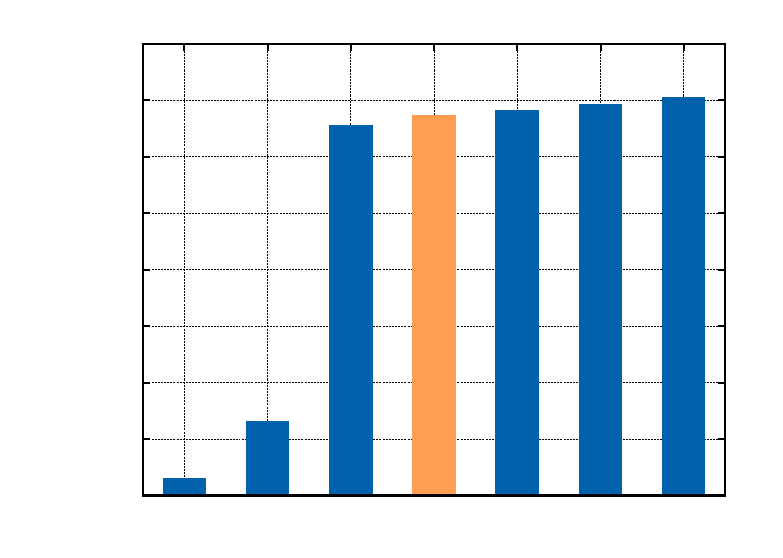
\includegraphics{eventdetectF1}}%
    \gplfronttext
  \end{picture}%
\endgroup

\caption{}
\label{fig:componentTime}
\end{figure}


\section{Scene Recognition Evaluation}
\subsection{Evaluation Data}
After we have done event detection, we use the previous proposed scene inference method to do scene recognition. 
In this section, a 10-scenes evaluation experiment are carried out for evaluating our system's performance.\\ 

The 10 scenes we used in this evaluation is \textit{bathroom, beach, concert, forest, kitchen, office, park, restaurant, street, subway station}. 
These scenes are chosen both covering indoor and outdoor, quiet and noisy environments. 
The testing clips we used are downloaded mainly from previously mentioned sound search engines, and there is 10 clips for each scene, i.e., 100 in total. \\ 

\subsection{Baseline systems}
In this evaluation, we need to compare our systems with other systems. 
And this requires getting existing audio scene recognition system with source code, since we are going to train on different scenes. 
Luckily, IEEE AASP Challenge has a scene classification part\footnote{\url{http://c4dm.eecs.qmul.ac.uk/sceneseventschallenge/}}, and source code for sume of the submitted systems\footnote{\url{https://code.soundsoftware.ac.uk/projects/dcase2013submissions}} are available for downloading. 
On the website, there are 4 scene classification systems and one baseline scene classifier. 
Because of some programming issues, we choose 2 classification systems, together with the baseline scene classifier for comparison. 
Table \ref{table:systems} shows a summary of the systems used for comparison and our systems. 

\begin{table}[htb]
\caption{Summary of systems}
\begin{tabular}{ll}
\toprule
 Code & Method \\
\bottomrule
 Baseline & MFCCs, classified with a bag-of-frames approach \\ 
 RNH & Recurrence Quantification Analysis to MFCC time-series, classified by SVM \\ 
 GSR & 6669 features, classifed using SVM within 4-second window, then majority voting \\
 Our & MFCCs, dynamic segmentation, classified with GMM \\ 
\bottomrule
\end{tabular}
\label{table:systems}
\end{table}

\subsection{Evaluation Result}
Table \ref{table:ac} show the recognition accuracy for each audio scenes. 

\begin{table}[htbp]
\centering
\resizebox{0.95\textwidth}{!}{
\begin{tabular}{lccccccccccc}
\toprule
     & bathroom & beach & concert & forest & kitchen & office & park & restaurant & street & subway station & Average \\
\bottomrule
Baseline & $60\%$ & $40\%$ & $60\%$ & $40\%$ & $10\%$ & $40\%$ & $60\%$ & $30\%$ & $60\%$ & $70\%$ & $47\%$\\
RNH1 & $30\%$ & $40\%$ & $70\%$ & $40\%$ & $20\%$ & $30\%$ & $50\%$ & $50\%$ & $70\%$ & $50\%$ & $45\%$ \\
RNH2 & $20\%$ & $40\%$ & $70\%$ & $40\%$ & $40\%$ & $30\%$ & $50\%$ & $40\%$ & $70\%$ & $60\%$ & $46\%$ \\
GSR & $60\%$ & $50\%$ & $90\%$ & $50\%$ & $30\%$ & $60\%$ & $60\%$ & $60\%$ & $70\%$ & $80\%$ & $61\%$ \\
Our & $80\%$ & $60\%$ & $60\%$ & $40\%$ & $50\%$ & $100\%$ & $30\%$ & $0\%$ & $100\%$ & $20\%$ & $54\%$ \\
\bottomrule
\end{tabular}
}
\caption{Recognition accuracy for 10 audio scenes}
\label{table:ac}
\end{table}

\begin{figure}[htb]
\centering
% GNUPLOT: LaTeX picture with Postscript
\begingroup
  \makeatletter
  \providecommand\color[2][]{%
    \GenericError{(gnuplot) \space\space\space\@spaces}{%
      Package color not loaded in conjunction with
      terminal option `colourtext'%
    }{See the gnuplot documentation for explanation.%
    }{Either use 'blacktext' in gnuplot or load the package
      color.sty in LaTeX.}%
    \renewcommand\color[2][]{}%
  }%
  \providecommand\includegraphics[2][]{%
    \GenericError{(gnuplot) \space\space\space\@spaces}{%
      Package graphicx or graphics not loaded%
    }{See the gnuplot documentation for explanation.%
    }{The gnuplot epslatex terminal needs graphicx.sty or graphics.sty.}%
    \renewcommand\includegraphics[2][]{}%
  }%
  \providecommand\rotatebox[2]{#2}%
  \@ifundefined{ifGPcolor}{%
    \newif\ifGPcolor
    \GPcolorfalse
  }{}%
  \@ifundefined{ifGPblacktext}{%
    \newif\ifGPblacktext
    \GPblacktexttrue
  }{}%
  % define a \g@addto@macro without @ in the name:
  \let\gplgaddtomacro\g@addto@macro
  % define empty templates for all commands taking text:
  \gdef\gplbacktext{}%
  \gdef\gplfronttext{}%
  \makeatother
  \ifGPblacktext
    % no textcolor at all
    \def\colorrgb#1{}%
    \def\colorgray#1{}%
  \else
    % gray or color?
    \ifGPcolor
      \def\colorrgb#1{\color[rgb]{#1}}%
      \def\colorgray#1{\color[gray]{#1}}%
      \expandafter\def\csname LTw\endcsname{\color{white}}%
      \expandafter\def\csname LTb\endcsname{\color{black}}%
      \expandafter\def\csname LTa\endcsname{\color{black}}%
      \expandafter\def\csname LT0\endcsname{\color[rgb]{1,0,0}}%
      \expandafter\def\csname LT1\endcsname{\color[rgb]{0,1,0}}%
      \expandafter\def\csname LT2\endcsname{\color[rgb]{0,0,1}}%
      \expandafter\def\csname LT3\endcsname{\color[rgb]{1,0,1}}%
      \expandafter\def\csname LT4\endcsname{\color[rgb]{0,1,1}}%
      \expandafter\def\csname LT5\endcsname{\color[rgb]{1,1,0}}%
      \expandafter\def\csname LT6\endcsname{\color[rgb]{0,0,0}}%
      \expandafter\def\csname LT7\endcsname{\color[rgb]{1,0.3,0}}%
      \expandafter\def\csname LT8\endcsname{\color[rgb]{0.5,0.5,0.5}}%
    \else
      % gray
      \def\colorrgb#1{\color{black}}%
      \def\colorgray#1{\color[gray]{#1}}%
      \expandafter\def\csname LTw\endcsname{\color{white}}%
      \expandafter\def\csname LTb\endcsname{\color{black}}%
      \expandafter\def\csname LTa\endcsname{\color{black}}%
      \expandafter\def\csname LT0\endcsname{\color{black}}%
      \expandafter\def\csname LT1\endcsname{\color{black}}%
      \expandafter\def\csname LT2\endcsname{\color{black}}%
      \expandafter\def\csname LT3\endcsname{\color{black}}%
      \expandafter\def\csname LT4\endcsname{\color{black}}%
      \expandafter\def\csname LT5\endcsname{\color{black}}%
      \expandafter\def\csname LT6\endcsname{\color{black}}%
      \expandafter\def\csname LT7\endcsname{\color{black}}%
      \expandafter\def\csname LT8\endcsname{\color{black}}%
    \fi
  \fi
  \setlength{\unitlength}{0.0500bp}%
  \begin{picture}(7200.00,5040.00)%
    \gplgaddtomacro\gplbacktext{%
      \csname LTb\endcsname%
      \put(814,440){\makebox(0,0)[r]{\strut{} 0}}%
      \csname LTb\endcsname%
      \put(814,1059){\makebox(0,0)[r]{\strut{} 10}}%
      \csname LTb\endcsname%
      \put(814,1679){\makebox(0,0)[r]{\strut{} 20}}%
      \csname LTb\endcsname%
      \put(814,2298){\makebox(0,0)[r]{\strut{} 30}}%
      \csname LTb\endcsname%
      \put(814,2917){\makebox(0,0)[r]{\strut{} 40}}%
      \csname LTb\endcsname%
      \put(814,3536){\makebox(0,0)[r]{\strut{} 50}}%
      \csname LTb\endcsname%
      \put(814,4156){\makebox(0,0)[r]{\strut{} 60}}%
      \csname LTb\endcsname%
      \put(814,4775){\makebox(0,0)[r]{\strut{} 70}}%
      \csname LTb\endcsname%
      \put(1563,220){\makebox(0,0){\strut{}Baseline}}%
      \csname LTb\endcsname%
      \put(2796,220){\makebox(0,0){\strut{}RNH1}}%
      \csname LTb\endcsname%
      \put(4029,220){\makebox(0,0){\strut{}RNH2}}%
      \csname LTb\endcsname%
      \put(5262,220){\makebox(0,0){\strut{}Our}}%
      \csname LTb\endcsname%
      \put(6495,220){\makebox(0,0){\strut{}GSR}}%
      \put(176,2607){\rotatebox{-270}{\makebox(0,0){\strut{}Average Accuracy}}}%
    }%
    \gplgaddtomacro\gplfronttext{%
    }%
    \gplbacktext
    \put(0,0){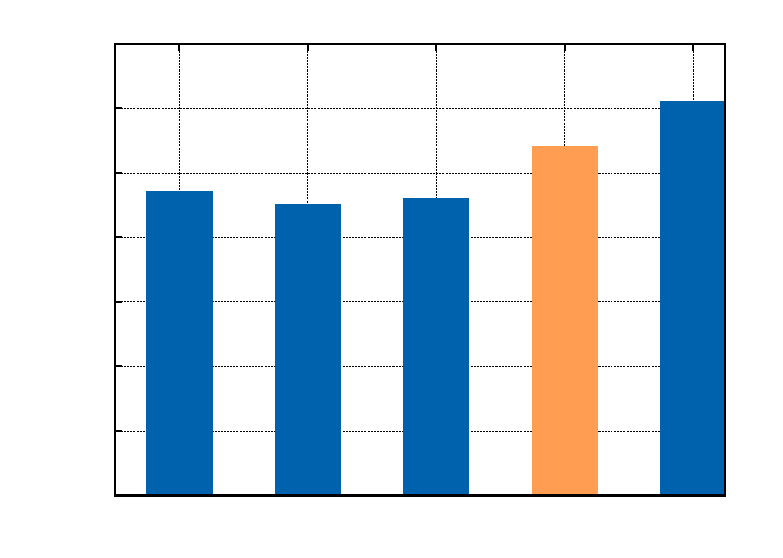
\includegraphics{sceneeval}}%
    \gplfronttext
  \end{picture}%
\endgroup

\caption{Recognition accuracy for 10 audio scenes}
\label{fig:sceneeval}
\end{figure}

\section{Summary}
